\documentclass{l3doc}
   \usepackage[T1]{fontenc}
	\usepackage{pdfpages}
	\usepackage{standalone}
	% \usepackage{gotham}
	% \usepackage{readprov}
	% 	\ReadPackageInfos{beamerthemegotham}
		\edef\GothamVersion{v1.2.1.c} %{\fileversion}
		\edef\GothamDate{2025-02-11} %{\filedate}


	\usepackage{parskip}
	\usepackage{setspace}
	\usepackage{xspace}
		\onehalfspacing

	\usepackage{xcolor}
		\definecolor{tPrim}{HTML}{00707F}   % Green-Blue
		\definecolor{tSec}{HTML}{5FA4B0}    % Green-Blue light
		\definecolor{tAccent}{HTML}{F07F3C} % Orange
		\definecolor{tGrey}{HTML}{E6E6E1}   % Grey-Beige

	\usepackage{listings}
		\lstset{%
			language=[LaTeX]{TeX},
			basicstyle=\ttfamily,
			keywordstyle=\color{tPrim}\bfseries,
			commentstyle=\color{tSec},
			stringstyle=\color{tSec},
			backgroundcolor=\color{white},
			numbers=none,
			numberstyle=\tiny\ttfamily,
			stepnumber=2,
			showspaces=false,
			showstringspaces=false,
			showtabs=false,
			frame=none,
			framerule=1pt,
			tabsize=2,
			rulesep=5em,
			captionpos=b,
			breaklines=true,
			breakatwhitespace=false,
			framexleftmargin=0em,
			framexrightmargin=0em,
			xleftmargin=0em,
			xrightmargin=0em,
			aboveskip=1em,
			belowskip=1em,
			morekeywords={\usetheme,\institute,\maketitle,\subtitle,
				\gothamset,
				\colorlet,\setbeamercolor,
				plain,\defbeamertemplate
			},
		}
		\lstMakeShortInline|

	\usepackage{hyperref}

		\setlength{\fboxsep}{0pt}%
	\usepackage{subcaption} % for subfigures
	\usepackage{cleveref} % for references

		\providecommand{\defopt}[1]{\underline{#1}}%{default: #1}%{\underline{#1}}
		\NewDocumentEnvironment{DescribeGothamOption}{ o m m m }{
			\DescribeOption{#2} % from l3doc
			\IfNoValueTF{#1}{
				% true => left empty intentionally
			}{
				\DescribeOption{% add extra info like added or updated dates to mimic 'function' env.
					\rule[2.5ex]{\linewidth}{0.3pt}
					\\[-3.5ex]
					{\scriptsize #1 \hfill\ }
				}
			}
			\begin{minipage}[t]{\textwidth}
				\textit{\textbf{\textcolor{tSec}{#3}}}\dotfill\,\defopt{#4}\par
				\begingroup
					\vspace{0.5em}
		}{
					\par
				\endgroup
			\end{minipage}
		}


%% =====================================================================
\title{\textsc{Gotham}\\ A modern, minimal-ish, versatile and extendable theme for Beamer}
\author{Romain NOEL \\ \url{romainoel@free.fr}}
\date{\GothamVersion~---~\GothamDate}

\providecommand{\themename}{\textbf{\textsc{Gotham}}\xspace}

%% =====================================================================


\begin{document}
\maketitle
\tableofcontents


%% ------------------------------------
\section{Introduction}
	Beamer is an awesome way to make presentations with \LaTeX, but its theme selection is surprisingly sparse. 
	The stock themes share an aesthetic that can be a little cluttered, while the few distinctive custom themes available are often specialized for a particular corporate or institutional brand.

	The goal of \themename is to provide a simple, modern Beamer theme suitable for anyone to use. 
	It tries to minimize noise and maximize space for content; some visual flourishes are offered as options.

	The final product provides a modern, elegant and versatile theme with a	high degree of customization.
	So it can easily be used to build a particular corporate or institutional brand theme on top of it.
 
	The implementation of this theme is strongly inspired from the excellent \href{https://github.com/matze/mtheme}{\textsc{Metropolis}} theme by Matthias Vogelgesang, from which it borrows numerous options.
	\themename's codebase lives on
	\href{https://gitlab.com/RomainNOEL/beamertheme-gotham} {Gitlab}.
	\newline
	If you have issues, find mistakes in the manual or want to help make the theme even better, please get in touch there.
	Any feature request, issue report or merge requests are welcome.


%% ------------------------------------
\section{Getting Started}
\subsection{Installing from CTAN}
	The latest stable version of \themename is available on
	\href{https://ctan.org/pkg/beamertheme-gotham}{CTAN} and should now be part of the usual \TeX\ distributions (\TeX\ Live, Mac\TeX\ , Mik\TeX\ ), under the name	\textit{beamertheme-gotham}. 
	It means that if your distribution is kept up-to-date, the package should normally be already installed on your system. 
	If this is not the case, consider updating the packages of your Tex distribution.

	For \TeX\ Live and Mac\TeX\ users, this usually means running
	\begin{lstlisting}
		tlmgr update --all
	\end{lstlisting}
	or if administrative privileges are required
	\begin{lstlisting}
		sudo tlmgr update --all
	\end{lstlisting}

	For Mik\TeX\ users, please refer to \href{https://miktex.org/howto/update-miktex}{the official Mik\TeX\ documentation}.


\subsection{Installing from Gitlab}
	If you want to use the cutting-edge development version of \themename, you can install it manually by following these steps:
	\begin{description}
		\item[Download the source] from
			\href{https://gitlab.com/RomainNOEL/beamertheme-gotham}{\themename repository}
			using |git clone| or as a 
			\href{https://gitlab.com/RomainNOEL/beamertheme-gotham/-/archive/master/beamertheme-gotham-master.zip}{zip archive} 
			of the latest development version.
		\item[Compile the style files] by running |l3build unpack| inside the downloaded	directory. 
			(Or run \LaTeX{} directly on |source/gothamtheme.ins|.)
		\item[Move the resulting |*.sty| files] to the folder containing your presentation. 
			To use \themename with many presentations, run
			|l3build install| or move the |*.sty| files to a folder in your \TeX{} path instead.
		\item[Use the theme] by declaring \lstinline|\usetheme{gotham}| in the preamble of your document.
	\end{description}

	\themename uses the l3build system to offer the following installation options for advanced users:
	\begin{description}
		\item[|l3build unpack|] builds the theme style files.
		\item[|l3build doc|] builds this documentation manual and the examples.
		\item[|l3build check|] builds the theme and manual.
		\item[|l3build clean|] removes the files generated by |l3build|.
		\item[|l3build install|] installs the theme into your local texmf folder.
		\item[|l3build uninstall|] removes the theme from your local texmf folder.
	\end{description}


% \subsection{Overleaf}
% 	\themename is therefore automatically supported for new documents. 
% 	If you want to switch older documents to use the \themename theme, you need to \href{https://www.overleaf.com/blog/new-feature-select-your-tex-live-compiler-version}{select
% 	TexLive 2021 or higher as your TeX Live version} (this may cause issues with other packages used in your presentation).

% 	In addition to that, a template project was created and is publicly available in the \href{https://www.overleaf.com/latex/templates/gotham-beamer-theme/wjyyzvdzqkgf}{Overleaf Gallery} to bootstrap your presentation.


%% ------------------------------------
\subsection{A Minimal Example}
	The following code shows a minimal example of a Beamer presentation using \themename, and the output generated is given on \cref{fig-minimal}.

	\begin{lstlisting}
		\documentclass{beamer}
		\usetheme{gotham} % Loads Gotham theme
		\title{A minimal example}
		\subtitle{using Gotham theme}
		\date{\today}
		\author{John DOE}
		\institute{Your university or company}
		
		\begin{document}
			\maketitle
			\section{First Section}
			\begin{frame}{First Frame}
				Hello world !
			\end{frame}
		\end{document}
	\end{lstlisting}

	\begin{figure}[htp]
		\centering
		\fbox{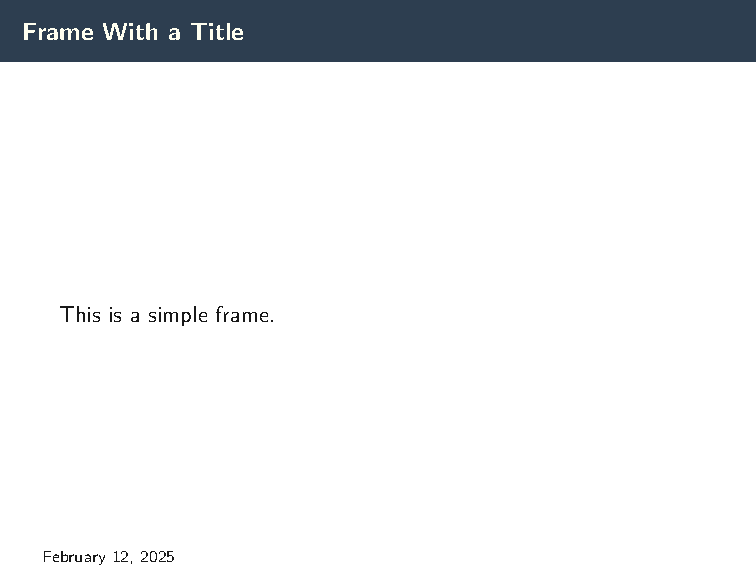
\includegraphics[width=0.7\textwidth]{gotham-exampleSimple.pdf}}
		\caption{A simple example.}
		\label{fig-minimal}
	\end{figure}


\subsection{Dependencies}
	\themename depends on the |beamer| class and the following standard packages:
	\begin{itemize}
		\item |tikz|
		\item |expl3|
		\item |xfp|
		\item |etoolbox|
		\item |ifxetex|
		\item |ifluatex|
	\end{itemize}

	For best results, we recommend installing the fonts
	\href{https://github.com/mozilla/Fira}{|Fira Sans|} and |Fira Mono| and compiling with \themename using XeLaTeX or LuaTeX.
	These are optional dependencies; \themename is compatible with (e.g.) pdf\LaTeX\ and will fall back to standard fonts if |Fira Sans| or |Fira Mono| is not installed.

	The packaged name of |Fira Sans| is |Fira Sans OT| in some Linux distributions; this case is automatically handled by \themename.


%% ------------------------------------
\section{Customization}
\subsection{Package options}
	\themename provides a number of options, which can be set using a key=value interface. 
	The primary way to set options is to provide a comma-separated list of option-value pairs when loading \themename in the preamble:
	\begin{lstlisting}[gobble=2]
		\usetheme[option1=value1, option2=value2, ...]{gotham}
	\end{lstlisting}

	Options can be changed at any time --- even mid-presentation ! --- with the |\gothamset| command.
	\begin{lstlisting}[gobble=2]
		\gothamset{option1=newvalue1, option2=newvalue2, ...}
	\end{lstlisting}

	The list of options is structured as shown in the following example.

	\begin{DescribeGothamOption}{option key}
	{list of possible values}{default}
		A short description of the option.
	\end{DescribeGothamOption}

	As \themename implementation is heavily inspired from the excellent
	\href{https://github.com/matze/mtheme}{\textsc{Metropolis}} theme by Matthias	Vogelgesang, many of \textsc{Metropolis} options are also available in \themename.


\subsubsection{Font theme}
	\DescribeOption{format title}
	% \begin{DescribeGothamOption}{format title}
	% {regular, lower, upper, titlecase}{regular}{
	% 	A short description of the option.
	% \end{DescribeGothamOption}
	\DescribeOption{format subtitle}
	% \begin{DescribeGothamOption}{format subtitle}
	% {regular, lower, upper, titlecase}{regular}{
	% 	A short description of the option.
	% \end{DescribeGothamOption}
	\DescribeOption{format frametitle}
	% \begin{DescribeGothamOption}{format frametitle}
	% {regular, lower, upper, titlecase}{regular}{
	% 	A short description of the option.
	% \end{DescribeGothamOption}
	\DescribeOption{format framesubtitle}
	% \begin{DescribeGothamOption}{format framesubtitle}
	% {regular, lower, upper, titlecase}{regular}{
	% 	A short description of the option.
	% \end{DescribeGothamOption}
	\DescribeOption{format part}
	% \begin{DescribeGothamOption}{format part}
	% {regular, lower, upper, titlecase}{regular}{
	% 	A short description of the option.
	% \end{DescribeGothamOption}
	\DescribeOption{format section}
	% \begin{DescribeGothamOption}{format section}
	% {regular, lower, upper, titlecase}{regular}{
	% 	A short description of the option.
	% \end{DescribeGothamOption}
	\begin{DescribeGothamOption}{format subsection}
	{regular, lower, upper, titlecase}{regular}
		Individually controls the format/case of titles, subtitles, frametitle, framesubtitles, part, section and subsection titles.
		\vspace{6em}
	\end{DescribeGothamOption}

	\DescribeOption{shape title}
	% \begin{DescribeGothamOption}{shape title}
	% {regular, italic, smallcaps}{regular}{
	% 	A short description of the option.
	% \end{DescribeGothamOption}
	\DescribeOption{shape subtitle}
	% \begin{DescribeGothamOption}{shape subtitle}
	% {regular, italic, smallcaps}{regular}{
	% 	A short description of the option.
	% }\end{DescribeGothamOption}
	\DescribeOption{shape frametitle}
	% \begin{DescribeGothamOption}{shape frametitle}
	% {regular, italic, smallcaps}{regular}{
	% 	A short description of the option.
	% }\end{DescribeGothamOption}
	\DescribeOption{shape framesubtitle}
	% \begin{DescribeGothamOption}{shape framesubtitle}
	% {regular, italic, smallcaps}{regular}{
	% 	A short description of the option.
	% }\end{DescribeGothamOption}
	\DescribeOption{shape part}
	% \begin{DescribeGothamOption}{shape part}
	% {regular, italic, smallcaps}{regular}{
	% 	A short description of the option.
	% }\end{DescribeGothamOption}
	\DescribeOption{shape section}
	% \begin{DescribeGothamOption}{shape section}
	% {regular, italic, smallcaps}{regular}{
	% 	A short description of the option.
	% }\end{DescribeGothamOption}
	\begin{DescribeGothamOption}{shape subsection}
	{regular, italic, smallcaps}{regular}{
		Individually controls the shape/series of titles, subtitles, frametitle, framesubtitles, part, section and subsection titles.
		\vspace{6em}
	}\end{DescribeGothamOption}

	\begin{figure}[htb]
		\centering
		\begin{subfigure}[b]{0.475\textwidth}
			 \centering
			 \includegraphics[width=\linewidth]{gotham-test-035-a.png}
			 \caption{Example of |format~frametitle=titlecase, shape~frametitle=smallcaps, format~framesubtitle= lower, shape~framesubtitle=regular|.}
			 \label{fig-035-a}
		\end{subfigure}
		\begin{subfigure}[b]{0.475\textwidth}
			 \centering
			 \includegraphics[width=\linewidth]{gotham-test-035-b.png}
			 \caption{Example of |format~frametitle=lower, shape~frametitle=italic, format~framesubtitle= regular, shape~framesubtitle=italic|.}
			 \label{fig-035-b}
		\end{subfigure}
		\caption{Examples of format and shape settings.}
		\label{fig-035}
  \end{figure}


\subsubsection{Color theme}
	The included \themename color theme is used by default, but its colors can be	easily changed to suit your tastes. 
	All of the theme's styles are defined in terms of a few main colors:
	\begin{itemize}
		\item |colorA| The primary theme color, used for frametitle, standout and text if the appropriate options are selected.
	\end{itemize}

	An easy way to customize the theme is to redefine these colors using:
	\begin{lstlisting}
		\colorlet{colorPale}{gPaleYell} % BG in light/normal mode
		\colorlet{colorDark}{gDarkBlack} % FG in light/normal mode
		\colorlet{colorA}{gDarkTeal} % frametitle, standin.out,
		\colorlet{colorAreversed}{gLightTeal} % frametitle, standin.in,
		\colorlet{colorB}{gMidGrey} % gray BG : progress bar, blocks
		\colorlet{colorC}{gDeepYellOr} % progress bar
		\colorlet{colorD}{gLightOrange} % alert
		\colorlet{colorE}{gLightGreen} % example
	\end{lstlisting}

	\begin{DescribeGothamOption}{background}{light, dark, transparent}{transparent}{
		Controls weather the color of all headings (title page, frame title, etc.)	should be in black (|default|) or in a slightly darker shade of the theme color |theme|.
	}\end{DescribeGothamOption}

	\begin{DescribeGothamOption}{colorset}
	{red, anthracite}{anthracite}{% blue, green, orange, teal, 
		Predefined set colors (|colorA, colorB, ...|) leading to different ambiances.
	}\end{DescribeGothamOption}

	\begin{DescribeGothamOption}{block}{native, transparent, fill}{native}{
		Optionally adds a light grey background to block environments like |theorem| and |example|.
	}\end{DescribeGothamOption}


\subsubsection{Inner theme}
	\begin{DescribeGothamOption}{title page}
	{gotham~normal, gotham~reversed, gotham~dividedpic, gotham~splitvert, <your-name>}{gotham~normal}{
		By setting this option you can change the title page according predefined style or even set your own template.		
		If you want to use your own template, this latter should be previously defined with:
		\lstinline|\defbeamertemplate{title page}{<your-name>}{<your-defintion>}|.
	}\end{DescribeGothamOption}
	
	\begin{DescribeGothamOption}{watermark default}
	{on, off}{off}{
		Enable or disable the watermark background template by default (ie. without using |\begin{frame}[watermark]|).
	}\end{DescribeGothamOption}

	\begin{DescribeGothamOption}{watermark template}
	{gotham~draft, <your-name>}{gotham~draft}{
		Set the watermark background template to use when the |watermark| option is activated (by default or locally).
		If you want to use your own template, this latter should be previously defined with:
		\lstinline|\defbeamertemplate{background}{watermark/<your-name>}{<your-defintion>}|.
	}\end{DescribeGothamOption}


	\DescribeOption{standin template}
	% \begin{DescribeGothamOption}{standin template}
	% {list of possible values}{default}{
	% 	A short description of the option.
	% }\end{DescribeGothamOption}
	\begin{DescribeGothamOption}[added=2024-11-11]{standout template}
	{gotham, <your-name>}{gotham}{
		Set the standin and stantout template to use when the |standin| or |stantout| frame option is activated.
		If you want to use your own template, this latter should be previously defined with:
		\lstinline|\defbeamertemplate{standout}{<your-name>}{<your-defintion>}|.
	}\end{DescribeGothamOption}

	\DescribeOption{standin BG template}
	% \begin{DescribeGothamOption}{standin BG template}
	% {list of possible values}{default}{
	% 	A short description of the option.
	% }\end{DescribeGothamOption}
	\begin{DescribeGothamOption}[updated=2024-11-11]{standout BG template}
	{gotham, <your-name>}{gotham}{
		Since most of the time the standin and standout are only varying from their backgrounds, \themename{} offers the possibility to change only and simply these local background through this option.
		This option sets the standin and stantout background template to use when the |standin| or |stantout| frame option is activated.
		If you want to use your own template, this latter should be previously defined with:
		\lstinline|\defbeamertemplate{background}{standin/<your-name>}{<your-defintion>}|.
	}\end{DescribeGothamOption}


	\DescribeOption{partframe default}	
	% \begin{DescribeGothamOption}{partframe default}
	% {list of possible values}{default}{
	% 	A short description of the option.
	% }\end{DescribeGothamOption}
	\DescribeOption{sectionframe default}
	% \begin{DescribeGothamOption}{sectionframe default}
	% {list of possible values}{default}{
	% 	A short description of the option.
	% }\end{DescribeGothamOption}
	\DescribeOption{subsectionframe default}
	% \begin{DescribeGothamOption}{subsectionframe default}
	% {list of possible values}{default}{
	% 	A short description of the option.
	% }\end{DescribeGothamOption}
	\begin{DescribeGothamOption}{subsubsectionframe default}
	{on, off}{on}{
		Enable or disable the display of the part frame (section, subsection and subsubsection respectively) at each part (other respectively) increment.
		\vspace{1em}
	}\end{DescribeGothamOption}

	\DescribeOption{partframe template}
	% \begin{DescribeGothamOption}{partframe template}
	% {list of possible values}{default}{
	% 	A short description of the option.
	% }\end{DescribeGothamOption}
	\DescribeOption{sectionframe template}
	% \begin{DescribeGothamOption}{sectionframe template}
	% {list of possible values}{default}{
	% 	A short description of the option.
	% }\end{DescribeGothamOption}
	\DescribeOption{subsectionframe~template}
	% \begin{DescribeGothamOption}{subsectionframe template}
	% {list of possible values}{default}{
	% 	A short description of the option.
	% }\end{DescribeGothamOption}
	\begin{DescribeGothamOption}{subsubsectionframe~template}
	{gotham progressbar, gotham simple, gotham splitvert progressbar, gotham splitvert simple, gotham progressvert}{gotham progressbar}{
		Set the frame template to use when the |part| (or |section|, |subsection|, |subsubsection| respectively) frame option is activated (ie. using |\begin{frame}[part]|).
		If you want to use your own template, before giving its name to this option, your template should be defined with:
		\lstinline|\defbeamertemplate{part frame}{<your-name>}{<your-defintion>}|.
		% \vspace{3em}
	}\end{DescribeGothamOption}


	\begin{DescribeGothamOption}{tocframe template}
	{gotham simple, gotham bullet, <your-name>}{gotham bullet}{
		Set the table of contents template to use when the |toc| option is activated.
		If you want to use your own template, this latter should be previously defined with:
		% \lstinline|
		\begin{lstlisting}[gobble=6]
			\defbeamertemplate{part in toc}{<your-name>}{<your-defintion>}
			\defbeamertemplate{section in toc}{<your-name>}{<your-defintion>}
			\defbeamertemplate{subsection in toc shaded}{<your-name>}{<your-defintion>}
			\defbeamertemplate{subsubsection in toc shaded}{<your-name>}{<your-defintion>}
			\defbeamertemplate{background canvas}{toc/<your-name>}{<your-definition>}
			\defbeamertemplate{toc page}{<your-name>}{<your-defintion, set them now by exmaple>}
		\end{lstlisting}
		% |.
	}\end{DescribeGothamOption}

	\DescribeOption{parttocframe default}	
	% \begin{DescribeGothamOption}{parttocframe default}
	% {list of possible values}{default}{
	% 	A short description of the option.
	% }\end{DescribeGothamOption}
	\DescribeOption{sectiontocframe default}
	% \begin{DescribeGothamOption}{sectiontocframe default}
	% {list of possible values}{default}{
	% 	A short description of the option.
	% }\end{DescribeGothamOption}
	\DescribeOption{subsectiontocframe default}
	% \begin{DescribeGothamOption}{subsectiontocframe default}
	% {list of possible values}{default}{
	% 	A short description of the option.
	% }\end{DescribeGothamOption}
	\begin{DescribeGothamOption}{subsubsectiontocframe~default}
	{on, off}{on}{
		Enable or disable the display of the table of content frame after the part frame (section, subsection and subsubsection respectively) at each part (other respectively) increment.
		\vspace{1em}
	}\end{DescribeGothamOption}

	\DescribeOption{parttocframe template}
	% \begin{DescribeGothamOption}{parttocframe template}
	% {list of possible values}{default}{
	% 	A short description of the option.
	% }\end{DescribeGothamOption}
	\DescribeOption{sectiontocframe template}
	% \begin{DescribeGothamOption}{sectiontocframe template}
	% {list of possible values}{default}{
	% 	A short description of the option.
	% }\end{DescribeGothamOption}
	\DescribeOption{subsectiontocframe~template}
	% \begin{DescribeGothamOption}{subsectiontocframe template}
	% {list of possible values}{default}{
	% 	A short description of the option.
	% }\end{DescribeGothamOption}
	\begin{DescribeGothamOption}{subsubsectiontocframe~tem..}
	{gotham simple, gotham bullet, <your-name>}{gotham bullet}{
		Set the frame template to use when the table of contents at each new |part| (or |section|, |subsection|, |subsubsection| respectively).
		This new frame is internally using the |tocpart| frame option to activate the frame template.
		If you want to use your own template, before giving its name to this option, your template should be defined with:
		\lstinline|\defbeamertemplate{part frame}{<your-name>}{<your-defintion>}|.
		% \vspace{3em}
	}\end{DescribeGothamOption}

	% \begin{figure}[h!]
	% 	\begin{subfigure}[b]{0.3\textwidth}
	% 		\fbox{\includegraphics[width=\textwidth]{screenshots/layout_example-04.jpg}}
	% 		\caption*{plain (default)}
	% 	\end{subfigure}
	% 	\hspace{\fill}
	% 	\begin{subfigure}[b]{0.3\textwidth}
	% 		\fbox{\includegraphics[width=\textwidth]{screenshots/layout_example-05.jpg}}
	% 		\caption*{style1}
	% 	\end{subfigure}
	% 	\hspace{\fill}
	% 	\begin{subfigure}[b]{0.3\textwidth}
	% 		\fbox{\includegraphics[width=\textwidth]{screenshots/layout_example-06.jpg}}
	% 		\caption*{style2}
	% 	\end{subfigure}
	% \end{figure}


\subsubsection{Outer theme}
	\DescribeOption{sidebar~canvas~right~template}
	% \begin{DescribeGothamOption}{subsectiontocframe template}
	% {list of possible values}{default}{
	% 	A short description of the option.
	% }\end{DescribeGothamOption}
	\begin{DescribeGothamOption}{sidebar~canvas~left~template}
	{~gotham~filigrane, empty, <your-name>}{gotham~filigrane}{
		Setting templates for left and right sidebar canvas which are activated when giving the frame option |\begin{frame}[edging]|.
		If you want to use your own template, before giving its name to this option, your template should be defined with:
		\lstinline|\defbeamertemplate{sidebar canvas right}{default/<your-name>}{<your-defintion>}|
	}\end{DescribeGothamOption}

	\begin{DescribeGothamOption}{edging default}
	{on, off}{off}{
		The option |edging default=on| can enable the |sidebar canvas right| (and |sidebar canvas left|) templates on every frame; but it can still be turned off for specific frames when using the frame option |\begin{frame}[noedging]|.
	}\end{DescribeGothamOption}

	\begin{DescribeGothamOption}{frametitle template}
	{gotham~subsameline, gotham~subnewline, <your-name>}{gotham~subsameline}{
		Option to set the frametitle template.
		\themename{} offers one template that adds the subtitle on the same line (|gotham~subsameline|) and one that adds the subtitle on a new line (|gotham~subnewline|).
		If you want to use your own template, before giving its name to this option, your template should be defined with:
		\lstinline|\defbeamertemplate{frametitle}{default/<your-name>}{<your-defintion>}|
	}\end{DescribeGothamOption}

	\begin{DescribeGothamOption}{framesubtitle template}
	{gotham~subnewline, <your-name>}{gotham~subnewline}{
		Setting the template to use when the subtitle is on a new line.
		If you want to use your own template, before giving its name to this option, your template should be defined with:
		\lstinline|\defbeamertemplate{framesubtitle}{default/<your-name>}{<your-defintion>}|
	}\end{DescribeGothamOption}

	\begin{DescribeGothamOption}{frametitle continuation template}
	{gotham, beamer, tot, <your-name>}{gotham}{
		Setting the template that is used in the frametitle when a frame too long and is continued/broke into several frames (using the frame option |allowframebreaks|).
		If you want to use your own template, before giving its name to this option, your template should be defined with:
		\lstinline|\defbeamertemplate{frametitle continuation}{default/<your-name>}{<your-defintion>}|
	}\end{DescribeGothamOption}

	\begin{DescribeGothamOption}{numbering}{none, framenumber, totalframenumber, appendixframenumber, pagenumber, totalpagenumber, circle}{none}{
		Setting the template with the frame number at the bottom right of each slide.
	}\end{DescribeGothamOption}

	\begin{DescribeGothamOption}{footer template}
	{gotham, <your-name>}{gotham}{
		Setting the template that appears in the footer of the frame.
		|gotham| footer print the |shortdate| at right, the |shorttitle| in the middle and the |shortauthor| at left.
		Since in 16/9 the height is precious, |gotham| template also offers the possibility to rotate |shortdate| and |shortauthor| so they appear on sides.
		If you want to use your own template, before giving its name to this option, your template should be defined with:
		\lstinline|\defbeamertemplate{frame footer}{default/<your-name>}{<your-defintion>}|
	}\end{DescribeGothamOption}	

	\begin{DescribeGothamOption}{rotateFooter default}
	{on, off}{off}{
		Enable or disable the |rotateFooter| frame option by default (ie. without using |\begin{frame}[rotateFooter]| on every frame).
		If the option is activated, it can be deactivated locally using the frame option |\begin{frame}[noRotateFooter]|.
	}\end{DescribeGothamOption}

	\begin{DescribeGothamOption}{mini frames shape}
	{default (bullet from beamer), tick, box, gotham minibullet, gotham box, gotham minibox, <your-name>}{gotham~minibullet}{
		Setting the shape of the mini frames to use, if the mini frame bundle refers to it (which is usually the case).
		If you want to use your own template, before giving its name to this option, your template should be defined with:
		% \lstinline|\defbeamertemplate{frame~footer}{default/<your-name>}{<your-defintion>}|
		\begin{lstlisting}[gobble=6]
			\defbeamertemplate{mini frame}{<your-name>}{
				<your-defintion>
			}[action]{
				\setbeamersize{mini frame size=.1cm, mini frame offset=.05cm}
			}
			\defbeamertemplate{mini frame in current subsection}{<your-name>}{
				<your-defintion>
			}
		\end{lstlisting}
	}\end{DescribeGothamOption}

	\begin{DescribeGothamOption}{mini frames bundle}
	{gotham~mini, beamer, gotham~nano <your-name>}{gotham~mini}{
		Setting the set of symbols used in the mini frame navigation.
		If you want to use your own template, before giving its name to this option, your template should be defined with:
		% \lstinline|\defbeamertemplate{frame~footer}{default/<your-name>}{<your-defintion>}|
		\begin{lstlisting}[gobble=6]
			\defbeamertemplate{miniframe~home}{<your-name>}{<your-def>}
			\defbeamertemplate{miniframe~current~slide}{<your-name>}{<your-def>}
			\defbeamertemplate{miniframe~done~current~section}{<your-name>}{<your-def>}
			\defbeamertemplate{miniframe~todo~current~section}{<your-name>}{<your-def>}
			\defbeamertemplate{miniframe~done~other~section}{<your-name>}{<your-def>}
			\defbeamertemplate{miniframe~todo~other~section}{<your-name>}{<your-def>}
			\defbeamertemplate{miniframe~part}{<your-name>}{<your-def>}
			\defbeamertemplate{miniframe~section~current}{<your-name>}{<your-def>}
			\defbeamertemplate{miniframe~section~done}{<your-name>}{<your-def>}
			\defbeamertemplate{miniframe~section~todo}{<your-name>}{<your-def>}
			\defbeamertemplate{miniframe~subsection~current}{<your-name>}{<your-def>}
			\defbeamertemplate{miniframe~subsection~todo}{<your-name>}{<your-def>}
			\defbeamertemplate{miniframe~subsection~done}{<your-name>}{<your-def>}
		\end{lstlisting}
	}\end{DescribeGothamOption}

	\begin{DescribeGothamOption}{mini frames compress}
	{on, off}{on}{
		A shortcut for the beamer option |compress| that affects the mini frames.
	}\end{DescribeGothamOption}

	\begin{DescribeGothamOption}{mini frames nav spreading}
	{spreading, centering, left, right}{spreading}{
		Controls how the mini frame should spread in the navigation bar.
	}\end{DescribeGothamOption}

	\begin{DescribeGothamOption}{mini frames nav sectioning}
	{none, section, secsubsection}{none}{
		Setting the |section in head/foot| template that is used on top of the mini frame navigation bar.
	}\end{DescribeGothamOption}

	\begin{DescribeGothamOption}{mini frames nav position}
	{none, head, foot, left, right}{none}{
		Setting where the mini frame navigation bar should appear.
	}\end{DescribeGothamOption}

	\begin{DescribeGothamOption}{progressbar position}
	{none, head, frametitle, foot, circlehead, left, right}{none}{
		Setting where the progressbar should appear.
		The different positions are pretty obvious from their name, except for |circlehead|.
		This latter option is putting a circular progressbar around the frametitle-logo (from frametitle template defined with gotham theme).
		It worth noting that by doing so, the frametitle is using the command |\gothamInstituteLogoCircle| instead of |\gothamInstituteLogoSquare| which is used otherwise.
	}\end{DescribeGothamOption}

	\begin{DescribeGothamOption}{progressbar style}
	{rectangle, rounded box, moving circle, fixed circle}{rectangle}{
		Setting how the progressbar should appear.
		|rectangle| option is using sharp rectangle for the progressbar, while |rounded box| is using rounded box and adds the percentage of progression at its right.
		|moving circle| and |fixed circle| are concerning the option |progressbar position=circle| only.
		|moving circle| add the number of the frame in a circle moving (following) the progression of the bar, while |fixed circle| put this framenumber constantly at the right of the circular progressbar.
	}\end{DescribeGothamOption}

	\begin{DescribeGothamOption}{progressbar advancement}
	{tlbr, brlt}{tlbr}{
		Defines in which direction the progressbar should evolve.
		|tlbr| is the shortcut for: starting from the top left corner, it goes bottom then right, ie. anti-clockwise.
		|brtl| is the shortcut for: starting from the bottom right corner, it goes top then left, ie. clockwise.
	}\end{DescribeGothamOption}

	\begin{DescribeGothamOption}{progressbar mfn}
	{on, off}{off}{
		Enable or disable the display of the mini frame navigation bar within the progressbar.
	}\end{DescribeGothamOption}


\subsection{Setup all the options}
	\begin{lstlisting}
	\gothamset{
		% from font theme
		format title, shape title,
		format subtitle, shape subtitle,
		format frametitle, shape frametitle,
		format framesubtitle, shape framesubtitle,
		format part, shape part,
		format section, shape section,
		format subsection, shape subsection,
		% from color theme
		background, 
		block, 
		colorset,
		% from inner theme
		title page,
		watermark template, watermark default,
		standout template, standin template,
		standout BG template, standin BG template,
		partframe template, partframe default,
		sectionframe template, sectionframe default,
		subsectionframe template, subsectionframe default,
		subsubsectionframe template, subsubsectionframe default,
		tocframe template, 
		parttocframe template, parttocframe default,
		sectiontocframe template, sectiontocframe default,
		subsectiontocframe template, subsectiontocframe default,
		%subsubsectiontocframe template, subsubsectiontocframe default,
		% from outer theme
		sidebar canvas right template, sidebar canvas left template,
		edging default,
		frametitle template, framesubtitle template, frametitle continuation template,
		numbering, 
		rotateFooter default,
		footer template,
		mini frames shape, mini frames bundle, mini frames compress, mini frames nav spreading, 
		progressbar position, progressbar style, progressbar advancement, progressbar mfn,
	}
	\end{lstlisting}
	

\subsection{Frame options}
	Frame options are affecting the templates used on the current frame through the following syntax:
	\begin{lstlisting}
		\begin{frame}[option] ... \end{frame}
	\end{lstlisting}
	Below a description of the different frame options brought by \themename{}.

	\DescribeOption{noBGC}
		Apply an empty |background canvas| template.

	\DescribeOption{watermark}
	\DescribeOption{nowatermark}
		Apply (with |watermark|) or deactivated (|nowatermark| when \lstinline|\gothamset{watermark default=on}| was given) the |background| template, through %\\
		\lstinline|\defbeamertemplate{background}{watermark/<your-name>}{<your-def>}| and %\\
		\lstinline|\gothamset{watermark template=<your-name>}|.

	\DescribeOption{standout}
	\DescribeOption{standin}
		Apply the |standin| (and |standout| respectively) templates through the definition
		\lstinline|\defbeamertemplate{standin}{<your-name>}{<your-def>}| and the option \lstinline|\gothamset{standin BG template=<your-name>}|.

	\DescribeOption{toc}
		Appy the |toc| template defined by \lstinline|\gothamset{tocframe template=<your-name>}|.

	\DescribeOption{edging}
	\DescribeOption{noedging}
		Apply (with |edging|) or deactivated (|noedging| when \lstinline|\gothamset{edging default=on}| was given) the |sidebar canvas left| (and right respectively) template, through 
		\lstinline|\defbeamertemplate{sidebar canvas left}{default/<your-name>}{<your-def>}| (and right)
		and the option 
		\lstinline|\gothamset{sidebar canvas left template=<your-name>}| (and right).

	\DescribeOption{nologo}
	\DescribeOption{nofootline}
	\DescribeOption{nofooter}
		Apply empty |logo| (and |footline|, |footer| respectively) templates. 
		This can be convenient when extra space is needed.
		\vspace{1em}

	\DescribeOption{rotateFooter}
	\DescribeOption{noRotateFooter}
		Enable or disable the rotation of the elements in the |footer|.
		This can be convenient when extra space is needed in 16/9 mode especially.

	\DescribeOption{part}
	\DescribeOption{section}
	\DescribeOption{subsec}
	\DescribeOption{subsubsec}
		Apply \lstinline|\usebeamertemplate{part frame}|, (|section frame|, |subsection frame| and |subsubsection frame| respectively) templates.
		This makes more sense for internal use, but can be reused everywhere else.
		\vspace{2em}

	\DescribeOption{tocpart}
	\DescribeOption{tocsec}
	\DescribeOption{tocsubsec}
	\DescribeOption{tocsubsubsec}
		Apply \lstinline|\usebeamertemplate{toc part frame}|, (|toc section frame|, |toc subsection frame| and |toc subsubsection frame| respectively) templates.
		This makes more for internal use, but can be reused everywhere else.
		\vspace{1em}


%% ------------------------------------
\subsection{Commands for Customization}
	\themename{} defines some commands that can be used as hooks, ie., that can be redefined when needed.

	\begin{function}{\gothamInstituteLogoCircle[1][4ex]}
		\begin{arguments}
			\item |height| of the picture. 
		\end{arguments}
		Command to include the circular logo of your institute in the frametitle when using \lstinline|\gothamset{progressbar position=circlehead}|.
		For example, you redefine this command through:
		\begin{lstlisting}[gobble=6]
			\renewcommand{\gothamInstituteLogoCircle}[1][4ex]{
				\includegraphics[height=#1]{<your-logo-circular>}
			}
		\end{lstlisting}
	\end{function}

	\begin{function}{\gothamInstituteLogoSquare[1][4ex]}
		\begin{arguments}
			\item |height| of the picture. 
		\end{arguments}
		Command to include the circular logo of your institute in the frametitle.
		For example, you redefine this command through:
		\begin{lstlisting}[gobble=6]
			\renewcommand{\gothamInstituteLogoSquare}[1][4ex]{
				\includegraphics[height=#1]{<your-logo-square>}
			}
		\end{lstlisting}
	\end{function}

	\begin{function}{\gothamFrameSubtitleSep}
		Command defining the separator used between the frametitle and the subtitle.
	\end{function}

	\begin{function}{\gothamRightFiligrane, \gothamLeftFiligrane}
		Commands that are used by default in the |sidebar canvas right| (and left).
		This avoids the redefinition of the whole templates, especially since the |sidebar canvas right| is containing elements by default in Beamer theme (like the |logo|).
	\end{function}

	\begin{function}{\gothamtitlepagelogo}
		% \begin{arguments}
		% 	\item |height| of the picture. 
		% \end{arguments}
		The command to insert the institute logo(s) on title page.
		For example, you redefine this command through:
		\begin{lstlisting}[gobble=6]
			\renewcommand{\gothamtitlepagelogo}{
				\includegraphics[height=#1]{<your-logo-on-titlepage>}
			}
		\end{lstlisting}
	\end{function}

	\begin{function}{\gothamtitlepagebg}
		% \begin{arguments}
		% 	\item |height| of the picture. 
		% \end{arguments}
		The command to insert the background title page.
		For example, you redefine this command through:
		\begin{lstlisting}[gobble=6]
			\renewcommand{\gothamtitlepagebg}{
				\includegraphics[height=#1]{<your-background-on-titlepage>}
			}
		\end{lstlisting}
	\end{function}

	\begin{function}{\partContentName, \secContentName, \subsecContentName}
		% \begin{arguments}
		% 	\item |height| of the picture. 
		% \end{arguments}
		The command to change the title of frames containing part's (or section or subsection) table of contents.
		For example, you redefine this command through:
		\begin{lstlisting}[gobble=6]
			\renewcommand{\partContentName}{Part's agenda}
		\end{lstlisting}
	\end{function}

	\begin{function}[added = 2025-01-06]{\partpageOptions, \sectionpageOptions, \subsectionpageOptions, \subsubsectionpageOptions}
		% \begin{arguments}
		% 	\item |height| of the picture. 
		% \end{arguments}
		The commands to change the options of frames containing part's title (or section or subsection) at its start.
		For example, you redefine this command through:
		\begin{lstlisting}[gobble=6]
			\renewcommand{\partpageOptions}{plain}
		\end{lstlisting}
	\end{function}

	\begin{function}[added = 2025-01-06]{\partpageTocOptions, \sectionpageTocOptions, \subsectionpageTocOptions}%, \subsubsectionpageTocOptions
		% \begin{arguments}
		% 	\item |height| of the picture. 
		% \end{arguments}
		The command to change the options of frames containing part's (or section or subsection) table of contents.
		For example, you redefine this command through:
		\begin{lstlisting}[gobble=6]
			\renewcommand{\partpageTocOptions}{nofooter}
		\end{lstlisting}
	\end{function}

	\begin{function}[added = 2025-01-06]{\partTocOptions, \sectionTocOptions, \subsectionTocOptions}%, \subsubsectionTocOptions
		% \begin{arguments}
		% 	\item |height| of the picture. 
		% \end{arguments}
		The command to change the options for part's (or section or subsection) table of contents at the beginning of this part.
		For example, you redefine this command through:
		\begin{lstlisting}[gobble=6]
			\renewcommand{\sectionTocOptions}{
				currentsection, hideallsubsections
			}
		\end{lstlisting}
	\end{function}

	\begin{variable}{gothamZerosectionframes}
		Boolean variable to flag if they are frame in a zeroth section.
		This variable helps to adapt the spreading of |mini frames nav| bar.
		This variable is automatically set if the spread is set correctly at the beginning of the presention. 
		If the spreading or the mini frame nav is disable at the zeroth section then reactivated latter, it might create unwanted spreading.
		In such situation the variable has to be set manually to correct the spreading.
		You change its value with |\booltrue{gothamZerosectionframes}|.
	\end{variable}

	\begin{variable}{darkBG, transparentBG}
		A boolean variables that are true with the background mode.
		It can be useful when you want to apply different codes according to the background you are on.
		You can use it as in the following example:
		\begin{lstlisting}[gobble=6]
			\ifbool{darkBG}{code to apply on dark background}{other code for light or transparent backgrounds}
		\end{lstlisting}
	\end{variable}

	\begin{function}[updated=2024-11-11]{\gothamHookFooter}
		% \begin{arguments}
		% 	\item |height| of the picture. 
		% \end{arguments}
		The command to add elements (like a logo) in the footer without redefining it completely.
		For example, you redefine this command through:
		\begin{lstlisting}[gobble=6]
			\renewcommand{\gothamHookFooter}{
				\usebeamertemplate{instituteLogo}
			}
		\end{lstlisting}
	\end{function}

	\begin{function}[updated=2024-11-11]{\gothamHookPostColorBGSet}
		% \begin{arguments}
		% 	\item |height| of the picture. 
		% \end{arguments}
		The command to change the colors that are related to the background color setting (ie. frametitle, standin, standout and titlepage).
		For example, you redefine this command through:
		\begin{lstlisting}[gobble=6]
			\renewcommand{\gothamHookPostColorBGSet}{
				\colorlet{colorFrametitle}{yourColor}
				\colorlet{colorStandout}{yourColor}
				\colorlet{colorStandin}{yourColor}
				\colorlet{colorTitlepage}{yourColor}
				\setbeamercolor{frametitle}{fg=yourRed, bg=}
			}
		\end{lstlisting}
	\end{function}
	

\subsection{Color Customization}
	The included \themename color theme is used by default, but its colors can be easily changed to suit your tastes. 
	All of the theme's styles are defined in terms of three Beamer colors:
	\begin{itemize}
		 \item |normal text| (dark fg, light bg)
		 \item |alerted text| (colored fg, should be visible against dark or light)
		 \item |example text| (colored fg, should be visible against dark or light)
	\end{itemize}
	
	An easy way to customize the theme is to redefine these colors using
	\begin{lstlisting}
		\setbeamercolor{ ... }{ fg= ... , bg= ... }
	\end{lstlisting}
	in your preamble. 
	For greater customization, you can redefine any of the other stock Beamer colors. 
	In addition to the stock colors the theme defines a number of \themename specific colors, which can also be redefined to your liking.
	
	\begin{lstlisting}
		\setbeamercolor{progress bar}{ ... }
		\setbeamercolor{title separator}{ ... }
		\setbeamercolor{progress bar in head/foot}{ ... }
		\setbeamercolor{progress bar in section page}{ ... }
	\end{lstlisting}
	
	
\subsection{Font Customization}
	The default font for \themename is |Fira|. 
	This can be easily changed using the standard font selection commands of the \textsf{fontspec} package. 
	So if you prefer, for example, the \href{http://font.ubuntu.com}{|Ubuntu|} font family, just add the following two commands after loading the \themename theme.
	
	\begin{lstlisting}
		\setsansfont{Ubuntu}
		\setmonofont{Ubuntu Mono}
	\end{lstlisting}
	
	If you are expecting to present in a large room or with an underpowered	projector, you may want to change the font to a heavier weight of Fira to maximize readability.
	
	\begin{lstlisting}
		\setsansfont[BoldFont={Fira Sans SemiBold}]{Fira Sans Book}
	\end{lstlisting}
	
	
\subsubsection{Old style figures}
	The regular \textsf{fontspec} mechanism for changing glyph appearance also applies to this theme. 
	If you want to have old style figures in the text but regular lined figures for math, you could add the following to your preamble:
	\begin{lstlisting}
		\usefonttheme{professionalfonts}   % required for mathspec
		\usepackage{mathspec}
		\setsansfont[BoldFont={Fira Sans},
						Numbers={OldStyle}]{Fira Sans Light}
		\setmathsfont(Digits)[Numbers={Lining, Proportional}]{Fira Sans Light}
	\end{lstlisting}


% \subsection{Backgrounds available}
% 	xx


\subsection{Length Customization}
	\begin{variable}{\gothamFrametitleToppading,
		\gothamFrametitleBottompading,
		\gothamFrametitleLeftpading,
		\gothamFrametitleRightpading} 
		Lengths controling the padding around the frametitle.
	\end{variable}

	\begin{variable}{\gothamFramesubtitleStrutend} 
		Lengths controling the padding around the frametitle.
	\end{variable}

	\begin{variable}{\sidebarRightHOffset, \sidebarLeftHOffset} 
		Length controling the horizontal and vertical offset in order to position |\gothamRightFiligrane| (respectively |\gothamLeftFiligrane|) when using the default sidebar canvas (right and left) from \themename.
	\end{variable}
	
	\begin{variable}{\gothamFootlineRuleLeftPadding, \gothamFootlineRuleHeight, \gothamFootlineRuleLength} 
		|\gothamFootlineRuleLeftPadding| is controlling the horizontal space between the left border of the page and the left side of the rule.
		|\gothamFootlineRuleHeight| controls the height and | \gothamFootlineRuleLength| the length of the rule used to delimit the footer.
	\end{variable}

	\begin{variable}[updated=2024-11-11]{\gothamFootlineHRightOffset, \gothamFootlineVOffset, \gothamFootlineHeight, \gothamFootlineDepth} 
		|\gothamFootlineHRightOffset| is controlling the horizontal space between the right border of the page and the side of the footline.
		|\gothamFootlineVOffset| is controlling space between to bottom of the text (or the footnote) and the footline.
		|\gothamFootlineHeight| and |\gothamFootlineDepth| are controlling the height and depth of the footline baseline.
	\end{variable}

	\begin{variable}{\gothamLeftFooterPadding, \gothamRightFooterPadding, \gothamFooterHOffset} 
		|\gothamLeftFooterPadding| is controlling the horizontal space between the left border of the page and the side of the footer.
		|\gothamRightFooterPadding| is controlling the horizontal space between the right the footer and the page number.
		|\gothamFooterHOffset| is controlling the horizontal space between the footer and the bottom of the page (or the progressbar).
	\end{variable}

	\begin{variable}{\gothamHposLeftRotFooter, \gothamHposRightRotFooter, \gothamVposLeftRotFooter, \gothamVposRightRotFooter} 
		Lengths that are controlling the horizontal and vertical positioning of the left and right elements of the rotated footer.
	\end{variable}	
	
	\begin{variable}{\gothamProgressCircHeight, \gothamCounterCircleRadius, \gothamProgressCircBorderWidth} 
		Lengths controlling the aspect of |progress circle|.
		|\gothamProgressCircHeight| is controlling the inner height of the circle (related to its diameter).
		|\gothamCounterCircleRadius| is controlling the size of the counter circle containing the frame number.
		|\gothamProgressCircBorderWidth| is controlling width of the progress circle.
	\end{variable}

	\begin{variable}{\gothamProgressHeadFootLineheight} 
		|\gothamProgressHeadFootLineheight| is controlling the height of the progress bar in "normal" frames (or its width when it is put in side bars).
	\end{variable}

	\begin{variable}{\gothamCircleNumberingVshift, \gothamCircleNumberingHshift} 
		Lengths controlling the vertical and horizontal positioning of the |circle| frame numbering template.
	\end{variable}

	\begin{variable}{\sectionhoffset, \gothamProgressSectionHeight} 
		|\sectionhoffset| controls the horizontal offset of the (section title + progress bar) block. 
		Can be useful when extra stuff wants to be displayed on sides of the block.
		The default value is 0pt.

		|\gothamProgressSectionHeight| controls the height of the progress bar used in part/section/subsection/subsubsection frames (when progress bar are used).
	\end{variable}

	\begin{figure}[htp]
		\centering
		\fbox{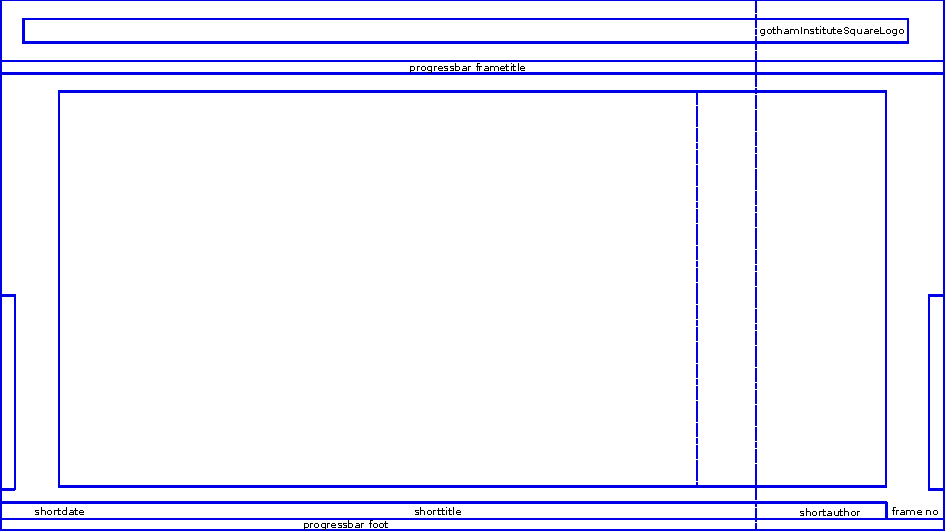
\includegraphics[width=0.7\textwidth]{gotham-layout.pdf}}
		\caption{The layout used by \themename.}
	\end{figure}


%% ------------------------------------
\section{Tips \& Tricks}
\subsection{Backup Slides}
	Speakers will often include extra slides at the end of their presentation to refer to during audience questions. 
	One easy way to do this is to include the	\verb|appendixnumberbeamer| package in your preamble and call \verb|\appendix| before your backup slides.

	\themename will automatically turn off slide numbering for slides in the appendix.


\subsection{Sources of inspiration}
	Many Beamer themes have been used as sources of inspiration to build \themename{}:
	\begin{itemize}
		\item \url{https://github.com/matze/mtheme} for dark/light theme and standout page.
		\item \url{https://github.com/hamaluik/Beamer-Theme-Execushares} and
			\\ \url{https://github.com/pcafrica/focus-beamertheme} for titlepage and sectionpage.
		\item \url{https://github.com/LukasPietzschmann/awesome-beamer} for titlepage.
		\item \url{https://github.com/luistar/unina-beamer/tree/master} and
			\\ \url{https://github.com/jkjaer/aauLatexTemplates/tree/master/aauBeamer/aausimple} for circlehead progress bar.
		\item \url{https://github.com/povanberg/flux-beamer} for toc.
		\item \url{https://github.com/fliptanedo/FlipBeamerTheme} for numbering circled fraction.
		\item \url{https://gitlab.com/RomainNOEL/latex3_template_pkg} for LateX3 template.
	\end{itemize}


%% ------------------------------------
\section{Known Issues}

\subsection{Title formats}
\label{sec:titleformats}
	Be aware that not every font supports small caps, so the |smallcaps| or |upper| options may not work if you use a font other than |Fira Sans|.
	In particular, the Computer Modern sans-serif typeface, which is used when \themename is compiled with pdf\LaTeX, does not have a small-caps variant.
	
	The title format options |upper| and |smallcaps| are quite nice from an aesthetic point of view, but their use of |\MakeLowercase| and
	|\MakeUppercase| can cause unexpected problems. 
	For example:
	\begin{itemize}
		\item Some commands, like |\\|, do not work inside |\MakeLowercase| and |\MakeUppercase|. 
		(See \href{https://github.com/matze/mtheme/issues/125}{\#125})
		\item Only alphabetic characters are affected by |\MakeLowercase|, so numerals and punctuation remain at full height. 
			This can spoil some of the aesthetic benefits of |upper|. 
			(See \href{https://github.com/matze/mtheme/issues/33}{\#33})
		\item |\MakeLowercase| and |\MakeUppercase| apply to math mode and |\scshape| does not. 
			This can easily introduce mathematical errors that are hard to catch.
		\item It is impossible to typeset symbols which are encoded as uppercase letters in a different font. 
			In particular, |\mathbb| and |\mathcal| letters will be replaced by other math glyphs. 
			(See \href{https://github.com/matze/mtheme/issues/153}{\#153})
	\end{itemize}
	
	The |smallcaps| and |upper| options are safe to use if your titles contain only alphabetic characters and do not require the expansion of any macros.
	
	
\subsection{Interactions with other color themes}
	\themename can be used along with any other Beamer color theme, such as |crane| or |seahorse|. 
	If you wish to do this, it is usually best to include the \themename subpackages individually so the \themename color theme is never loaded. 
	This will prevent conflicts between the \themename color theme and your preferred theme.
	
	For example, overriding the color theme as follows may not work as expected because |\usetheme{gotham}| loads the \themename color theme, which defines a relationship between the frametitle background and the primary palette of the theme. 
	Since |seahorse| assumes a different relationship between its palettes, the result is a grey, rather than periwinkle, frametitle background.
	
	\begin{lstlisting}
		\usetheme{gotham}
		\usecolortheme{seahorse}
	\end{lstlisting}
	
	The correct colors are chosen if the \themename outer, inner, and font themes are loaded seperately:
	\begin{lstlisting}
		\useoutertheme{gotham}
		\useinnertheme{gotham}
		\usefonttheme{gotham}
		\usecolortheme{seahorse}   % or your preferred color theme
	\end{lstlisting}
	
	Please note that \themename may not use all the colors defined in your favourite Beamer color theme. 
	In particular, \themename does not set a background color for the title; this will cause issues when using color themes like |whale| which set a white foreground for the title.
	
	
\subsection{Notes on second screen}
	If you use the |[show notes on second screen]| option built into Beamer and compile with XeLaTeX, text on slides following the first section slide may be rendered in white instead of the regular color. 
	This is due to \href{http://tex.stackexchange.com/questions/288408/}{a bug} in Beamer or XeLaTeX itself. 
	You can work around it either by compiling with LuaTeX or by adding the following code to your preamble to reset the text color on each slide.
	
	\begin{lstlisting}
		\makeatletter
		\def\beamer@framenotesbegin{% at beginning of slide
			\usebeamercolor[fg]{normal text}
				\gdef\beamer@noteitems{}%
				\gdef\beamer@notes{}%
		}
		\makeatother
	\end{lstlisting}
	
	
\subsection{Standout frames with labels}
	Because the |standout| frame option creates a group to restrict the colour change to a single slide, labels defined after calling |standout| will stay local to the group. 
	In other words, the following may result in a ``label undefined'' error.
	\begin{lstlisting}
		\begin{frame}[standout, label=conclusion]{Conclusion}
			Awesome slide
		\end{frame}
	\end{lstlisting}
	
	To fix this problem, change the order of the keys in the frame.
	\begin{lstlisting}
		\begin{frame}[label=conclusion, standout]{Conclusion}
			Awesome slide
		\end{frame}
	\end{lstlisting}
	
	This error can be unwittingly triggered if you export your slides from Emacs Org mode, which automatically adds labels after frame options. 
	Alex Branham \href{https://github.com/matze/mtheme/issues/203}{offers} the following solution for Org mode users, using |org-set-property|.
	
	\begin{lstlisting}
		* Start of a frame
			:PROPERTIES:
			:BEAMER_opt: label=conclusion,standout
			:END:
	\end{lstlisting}
	
	
\subsection{Standout frames with Pandoc}
	With Pandoc versions prior 1.17.2 it was not possible to create standout frames because Pandoc only supported a specific list of frame attributes thus ignoring additional attributes such as |{.standout}|.


\subsection{Other issues}
	\begin{itemize}
		\item |enumitem| is not working with Beamer.
	\end{itemize}


\subsection*{Todo}
	List of thing that could be improved (any volunteer welcome):
	\begin{itemize}
		\item Reduce the number of @ .
		\item Rename a lot of length with gotham at the beginning of their name.
		\item Turn internal length into \_dim.
		\item Improve documentation.
		\item Add a hexagonal, wavy and add lengths on the blueprint layout backgrounds.
		\item Remove colors from tests inner and outer.
		\item Replace the |\setbeamertemplate{yy}[default/xx]| by |\__gotham_inner_set_template:nn{title~page}| or merge them  because the default values in dict/template are interesting but |\__gotham_inner_set_template| are simpler.	
		\item  add colorset more "blue-ish", "green-ish" ... from colorA etc.
		\item add Gotham to lists of Awesome Beamer themes.
	\end{itemize}


\section{License}
	\themename is licensed under the terms of the
	% \href{https://creativecommons.org/licenses/by-sa/4.0/}{Creative Commons	Attribution-ShareAlike 4.0} 
	\href{https://www.latex-project.org/lppl/lppl-1-3c/}{LaTeX project public license (LPPL) 1.3c} 
	license.


\end{document}
% EoF


% \begin{documentation}
% 	\begin{macro|function|variable}[updated|added=2025-02-25]{\nameMacro}
%  	\begin{syntax}
% 			\cs{nameMacro}\oarg{option1=value1, ...}\marg{tempkg} 
% 			\textrm{where the options are (default marked as} \defopt{default}\textrm{):}
% 			\meta{footer template} = \oarg{\defopt{tempkg} \textbar ... }
% 		\end{syntax}
% 		Description of |nameMacro| which xxx.
% 	\end{macro|function|variable}
% \end{documentation}
%%%% 
% \begin{implementation}
% 	\begin{macro|function|variable}[updated|added=2025-02-25]{\nameMacro}
% 		\begin{arguments}
% 			\item |width| Name of the option to add, this name should also correspond to the name of the environment followed by the suffix 'env'. 
% 		\end{arguments}
% 		Description
% 		\changes{v1.0.1}{2025-02-25}{original version}
% 		\UnitTested % NOT FOR VARIABLES OF FUNCTIONS
% 		\TestFiles{tempkg-test-xxx} % NOT FOR VARIABLES
%    \begin{macrocode}
%% MY CODE
%    \end{macrocode}
% 	\end{macro|function|variable}
% \end{implementation}



% \begin{implementation}
% 	\begin{macro}[updated|added=2025-02-25]{\nameMacro}
% 		\begin{arguments}
% 			\item |width| Name of the option to add, this name should also correspond to the name of the environment followed by the suffix 'env'. 
% 		\end{arguments}
% 		Description
% 		\changes{v1.0.1}{2025-02-25}{original version}
% 		\UnitTested % NOT FOR VARIABLES OF FUNCTIONS
% 		\TestFiles{tempkg-test-xxx} % NOT FOR VARIABLES
%    \begin{macrocode}
%% MY CODE
%    \end{macrocode}
% 	\end{macro}
% \end{implementation}